\documentclass[10pt]{article}
\usepackage{graphicx}

\graphicspath{ {image/pic}}
\title{Android Malware: Characterization and Evolution}
\author{Himaja Kethiri}
\date{Tuesday,February 8,2016}
\begin{document}
\maketitle
\section{Introduction}
In present days there is a huge usage of smartphones which shows impact on security in the form of malwares.The Android malware is the type of malware which we can see on android platforms.\\

The main aim of this publication is to analyze the malware samples and to provide security for the devices.In this we have discussed some characterization and Evolution of android malware.In this publication authors did research on android malware using 3 phases.\\

First,they have taken 1260 samples of malware and divided them into 49 families of different types of malware.They almost did research on huge samples of malwares which are currently exist in Android market.Second,they performed timeline analysis on these collected samples.The analysis of these samples. \\
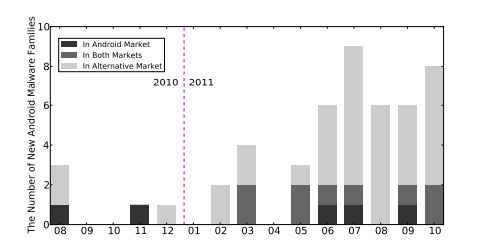
\includegraphics{pic.PNG}


Lastly,the malware samples are tested using android anti-malware softwares like AVG Antivirus free  etc.The results shows that the malware authors are able to create new malware(Hybrid malware) with the help of existing ones which is hard to detect for the user.These malwares are tested using anti-virus security softwares.\\

\section{Characterization}
     After analyzing the malware samples they have installed the malware onto phones using 3 strategies. 
\begin{enumerate}
\item Repackaging
\item Update attack
\item Drive-by download
\end{enumerate} 

\textbf{Repackaging:}
      In repackaging malware authors will download the most used applications. They will add some malwared payloads and re-assemle them so that no one can detect them as they are malicious.These malicious applications will be released as a new app.Now the users will download it which will effect the device. \\
      
\textbf{Update attack:}
      It will make use of famous applications same like Repackaging.But the only difference is the update attack will add only update field to the app instead of adding the payload.By displaying the update dialogue the user may think that it is the new version of application and he will allow the updates which inturns installs the malicious malware In to the device.\\
      
\textbf{Drive-by Download:}
     These type of attacks will infect the device while browsing.It will attract the user to download their interesting apps.It will attack the device by advertisements and page redirections.This attack is very useful  to hack the person bank information by asking him to download the mobile banking app.



\section{Evolution} 
      In the evolution of malware they have taken two samples named DroidKungFu and AnserverBot.The DroidKungFu malware was detected in June 2011.In this we have six versions.This malware consist of 473 samples.In this they observed that among six versions, four versions have encrypted data.This malware have another feature which is it can communicate with C and C servers by changing the server addresses which is hard to detect as malicious.AnserverBot was another malware which was discovered in Semptember 2011.This malware uses repackaging of applications.But,it tries to keep itself safe by checking whether these reassembled apps are altered or not.
\section{Conclusion}
     In this paper 1260 malware samples are analysed.The results shown that there is a rapid growth of malicious malwares detected in past years.These results will help us for further enhancement .


\end{document}
